\documentclass{standalone}
\usepackage{tikz}
\usetikzlibrary{patterns, positioning}
\usepackage[sfdefault]{ClearSans} %% option 'sfdefault' activates Clear Sans as the default text font
\usepackage[T1]{fontenc}

\begin{document}
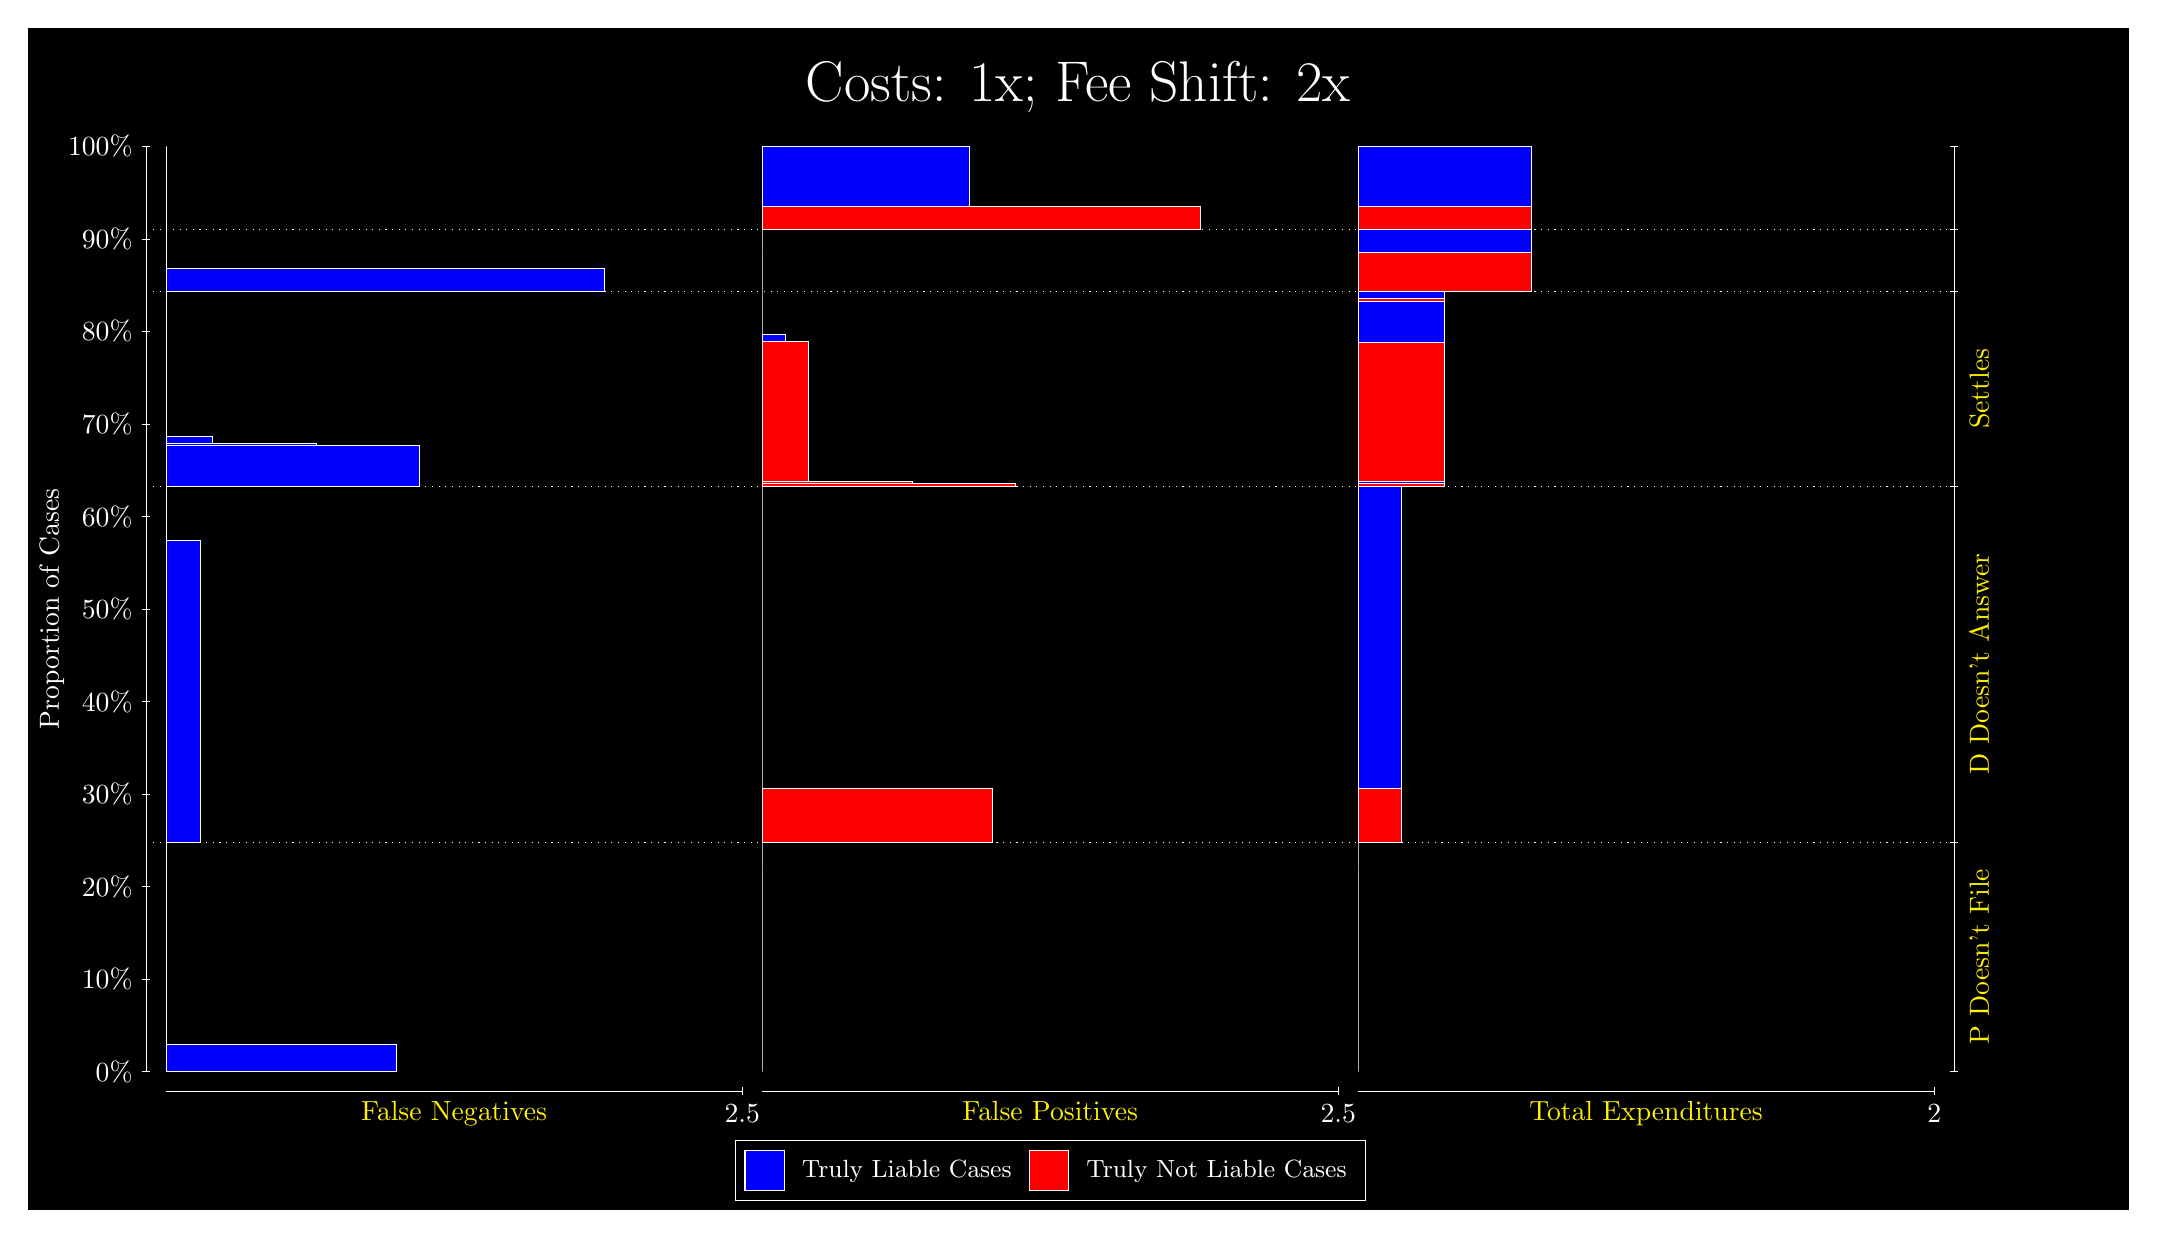
\begin{tikzpicture}
\draw[fill=black] (0,0) rectangle (26.667,15);
\draw[text=white] (0,13.5) rectangle (26.667,15) node[midway] {\huge Costs: 1x; Fee Shift: 2x};
\draw[white, very thin] (1.5,1.75) -- (1.5,13.5);
\node[rotate=90, text=white, anchor=center] at (0.3, 7.625) {Proportion of Cases};
\draw[white, very thin] (1.45,1.75) -- (1.55,1.75);
\node[text=white, anchor=east] at (1.45, 1.75) {0\%};
\draw[white, very thin] (1.45,2.925) -- (1.55,2.925);
\node[text=white, anchor=east] at (1.45, 2.925) {10\%};
\draw[white, very thin] (1.45,4.1) -- (1.55,4.1);
\node[text=white, anchor=east] at (1.45, 4.1) {20\%};
\draw[white, very thin] (1.45,5.275) -- (1.55,5.275);
\node[text=white, anchor=east] at (1.45, 5.275) {30\%};
\draw[white, very thin] (1.45,6.45) -- (1.55,6.45);
\node[text=white, anchor=east] at (1.45, 6.45) {40\%};
\draw[white, very thin] (1.45,7.625) -- (1.55,7.625);
\node[text=white, anchor=east] at (1.45, 7.625) {50\%};
\draw[white, very thin] (1.45,8.8) -- (1.55,8.8);
\node[text=white, anchor=east] at (1.45, 8.8) {60\%};
\draw[white, very thin] (1.45,9.975) -- (1.55,9.975);
\node[text=white, anchor=east] at (1.45, 9.975) {70\%};
\draw[white, very thin] (1.45,11.15) -- (1.55,11.15);
\node[text=white, anchor=east] at (1.45, 11.15) {80\%};
\draw[white, very thin] (1.45,12.325) -- (1.55,12.325);
\node[text=white, anchor=east] at (1.45, 12.325) {90\%};
\draw[white, very thin] (1.45,13.5) -- (1.55,13.5);
\node[text=white, anchor=east] at (1.45, 13.5) {100\%};

\draw[white, very thin] (24.457,1.75) -- (24.457,13.5);
\draw[white, very thin] (24.407,1.75) -- (24.507,1.75);
\node[anchor=west] at (24.407, 1.75) {};
\draw[white, very thin] (24.407,4.6639) -- (24.507,4.6639);
\node[anchor=west] at (24.407, 4.6639) {};
\draw[white, very thin] (24.407,9.1848) -- (24.507,9.1848);
\node[anchor=west] at (24.407, 9.1848) {};
\draw[white, very thin] (24.407,11.657) -- (24.507,11.657);
\node[anchor=west] at (24.407, 11.657) {};
\draw[white, very thin] (24.407,12.447) -- (24.507,12.447);
\node[anchor=west] at (24.407, 12.447) {};
\draw[white, very thin] (24.407,13.5) -- (24.507,13.5);
\node[anchor=west] at (24.407, 13.5) {};

\draw[white, very thin, fill=blue] (1.75,1.75) rectangle (4.6775,2.0976);
\draw[white, very thin, fill=red] (1.75,2.0976) rectangle (1.75,4.6639);
\draw[white, very thin, fill=blue] (1.75,4.6639) rectangle (2.1891,8.4993);
\draw[white, very thin, fill=red] (1.75,8.4993) rectangle (1.75,9.1848);
\draw[white, very thin, fill=blue] (1.75,9.1848) rectangle (4.9703,9.7068);
\draw[white, very thin, fill=blue] (1.75,9.7068) rectangle (3.6529,9.7323);
\draw[white, very thin, fill=blue] (1.75,9.7323) rectangle (2.3355,9.8236);
\draw[white, very thin, fill=red] (1.75,9.8236) rectangle (1.75,11.657);
\draw[white, very thin, fill=blue] (1.75,11.657) rectangle (7.3123,11.953);
\draw[white, very thin, fill=red] (1.75,11.953) rectangle (1.75,12.447);
\draw[white, very thin, fill=red] (1.75,12.447) rectangle (1.75,12.743);
\draw[white, very thin, fill=blue] (1.75,12.743) rectangle (1.75,13.5);
\draw[white, very thin, fill=red] (9.3189,1.75) rectangle (9.3189,4.3163);
\draw[white, very thin, fill=blue] (9.3189,4.3163) rectangle (9.3189,4.6639);
\draw[white, very thin, fill=red] (9.3189,4.6639) rectangle (12.246,5.3494);
\draw[white, very thin, fill=blue] (9.3189,5.3494) rectangle (9.3189,9.1848);
\draw[white, very thin, fill=red] (9.3189,9.1848) rectangle (12.539,9.2179);
\draw[white, very thin, fill=red] (9.3189,9.2179) rectangle (11.222,9.2511);
\draw[white, very thin, fill=red] (9.3189,9.2511) rectangle (9.9044,11.018);
\draw[white, very thin, fill=blue] (9.3189,11.018) rectangle (9.6116,11.109);
\draw[white, very thin, fill=blue] (9.3189,11.109) rectangle (9.3189,11.657);
\draw[white, very thin, fill=red] (9.3189,11.657) rectangle (9.3189,12.151);
\draw[white, very thin, fill=blue] (9.3189,12.151) rectangle (9.3189,12.447);
\draw[white, very thin, fill=red] (9.3189,12.447) rectangle (14.881,12.743);
\draw[white, very thin, fill=blue] (9.3189,12.743) rectangle (11.954,13.5);
\draw[white, very thin, fill=red] (16.888,1.75) rectangle (16.888,4.3163);
\draw[white, very thin, fill=blue] (16.888,4.3163) rectangle (16.888,4.6639);
\draw[white, very thin, fill=red] (16.888,4.6639) rectangle (17.437,5.3494);
\draw[white, very thin, fill=blue] (16.888,5.3494) rectangle (17.437,9.1848);
\draw[white, very thin, fill=red] (16.888,9.1848) rectangle (17.986,9.218);
\draw[white, very thin, fill=blue] (16.888,9.218) rectangle (17.986,9.2436);
\draw[white, very thin, fill=red] (16.888,9.2436) rectangle (17.986,11.01);
\draw[white, very thin, fill=blue] (16.888,11.01) rectangle (17.986,11.532);
\draw[white, very thin, fill=red] (16.888,11.532) rectangle (17.986,11.565);
\draw[white, very thin, fill=blue] (16.888,11.565) rectangle (17.986,11.657);
\draw[white, very thin, fill=red] (16.888,11.657) rectangle (19.083,12.151);
\draw[white, very thin, fill=blue] (16.888,12.151) rectangle (19.083,12.447);
\draw[white, very thin, fill=red] (16.888,12.447) rectangle (19.083,12.743);
\draw[white, very thin, fill=blue] (16.888,12.743) rectangle (19.083,13.5);
\draw[white, dotted] (1.5,4.6639) -- (24.457,4.6639);
\draw[white, dotted] (1.5,9.1848) -- (24.457,9.1848);
\draw[white, dotted] (1.5,11.657) -- (24.457,11.657);
\draw[white, dotted] (1.5,12.447) -- (24.457,12.447);
\draw[white, very thin] (1.75,1.5) -- (9.0689,1.5);
\node[text=yellow, anchor=north] at (5.4094, 1.5) {False Negatives};
\draw[white, very thin] (9.0689,1.45) -- (9.0689,1.55);
\node[text=white, anchor=north] at (9.0689, 1.45) {2.5};

\draw[white, very thin] (9.3189,1.5) -- (16.638,1.5);
\node[text=yellow, anchor=north] at (12.978, 1.5) {False Positives};
\draw[white, very thin] (16.638,1.45) -- (16.638,1.55);
\node[text=white, anchor=north] at (16.638, 1.45) {2.5};

\draw[white, very thin] (16.888,1.5) -- (24.207,1.5);
\node[text=yellow, anchor=north] at (20.547, 1.5) {Total Expenditures};
\draw[white, very thin] (24.207,1.45) -- (24.207,1.55);
\node[text=white, anchor=north] at (24.207, 1.45) {2};

\node[text=yellow, centered, rotate=90] at (24.777, 3.2069) {P Doesn't File};
\node[text=yellow, centered, rotate=90] at (24.777, 6.9243) {D Doesn't Answer};
\node[text=yellow, centered, rotate=90] at (24.777, 10.421) {Settles};



\draw (12.978300999999998,1.5) node[draw=none] (baseCoordinate) {};
\begin{scope}[align=center]
        \matrix[scale=0.5, draw=white, below=0.5cm of baseCoordinate, nodes={draw}, column sep=0.1cm]{
            \node[rectangle, draw, minimum width=0.5cm, minimum height=0.5cm, fill=blue] {}; &
            \node[draw=none, font=\small, text=white] (B) {Truly Liable Cases}; &
            \node[rectangle, draw, minimum width=0.5cm, minimum height=0.5cm, fill=red] {}; &
            \node[draw=none, font=\small, text=white] (B) {Truly Not Liable Cases}; \\
            };
\end{scope}

\end{tikzpicture}
\end{document}